\newpage
\section{MTB-2-AVR} \label{sec:mtb-2-avr}

Aby nebylo nutné všechny současné \gls{mtbuni} moduly vyměnit za moduly nové,
je třeba současné moduly povýšit tak, aby podporovaly nový protokol \gls{mtbbus} v4.
Kvůli omezenosti procesoru v~současných \gls{mtbuni} není možné tuto
úpravu provést pouze změnou firmwaru, viz \ref{sec:mtb_fail}.

Procesory v~současných \gls{mtbuni} modulech jsou
v~\gls{dil} patici. Nabízí se tedy přirozená cesta najít nový procesor
odpovídajícího rozložení pinů. Procesor, který by měl vyhovující rozložení pinů
a požadované parametry, bohužel neexistuje (uvažován byl například
\textit{ATtiny4313}). Proto se autor této práce vydal cestou výroby nástavné
desky, která se zasune do \gls{dil} patice současné \gls{mtbuni} desky
a~která na sobě bude mít \gls{smd} procesor.

Popsanou myšlenku realizuje deska \textit{MTB-2-AVR}, viz obrázek
\ref{fig:mtb-2-avr-alone}.

\begin{figure}[ht]
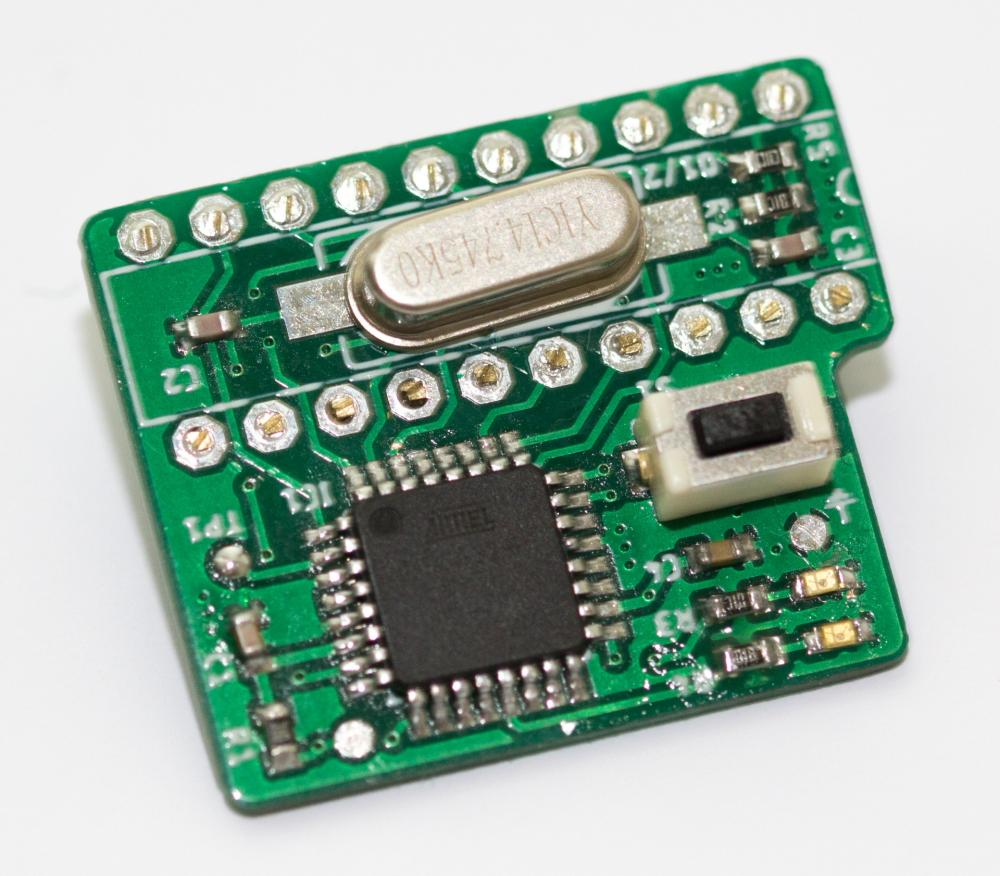
\includegraphics[width=0.4\textwidth]{data/uni-2-upgrade-alone.jpg}
\caption{Nástavná deska \textit{MTB-2-AVR}.}
\label{fig:mtb-2-avr-alone}
\end{figure}

\begin{figure}[ht]
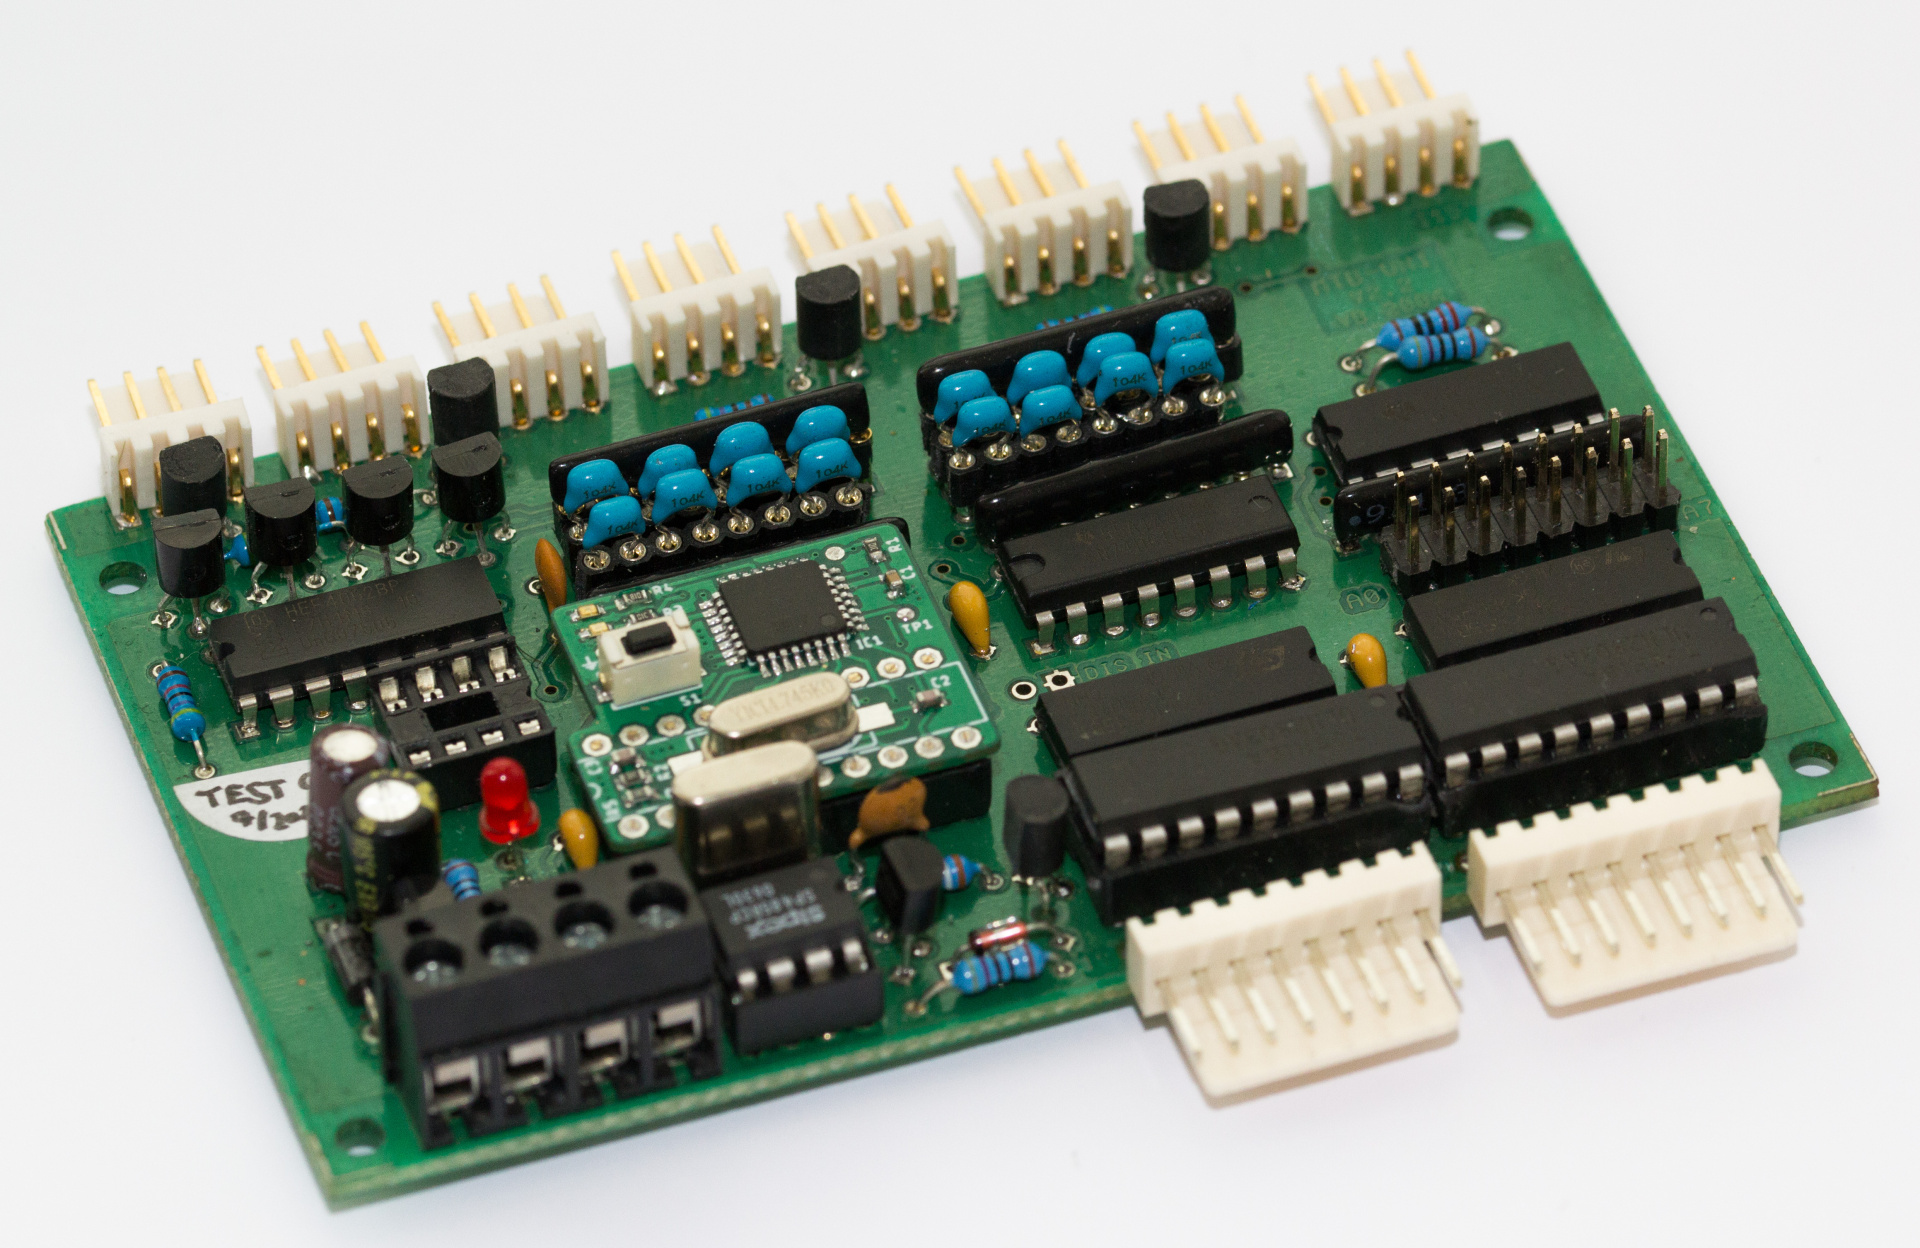
\includegraphics[width=0.8\textwidth]{data/uni-2-upgrade-all.jpg}
\caption{Nástavná deska \textit{MTB-2-AVR} v~modulu \gls{mtbuni} v2.}
\label{fig:mtb-2-avr-inside}
\end{figure}

Deska je navržena tak, aby se dala umístit místo procesoru libovolného z~modulů
\gls{mtbuni}, MTB-UNIm nebo MTB-TTL. Srdcem desky je procesor
\textit{ATmega328p} autorovy oblíbené architektury \textit{AVR}.
Konkrétně tento model byl zvolen, protože obsahuje dostatečnou kapacitu paměti
pro bootloader a~protože jej \textit{JLCPCB} má mezi \textit{basic} součástkami
(viz \ref{subsec:mtbusb:hardware}).

Schéma a \gls{dps} jsou vyvinuty jako openhardware projekt, dostupné
online\footnote{\url{https://github.com/kmzbrnoI/mtb-2-avr-pcb}} a~v~příloze
\ref{fig:mtb-uni-2-avr-sch}. Nástavná \gls{dps} obsahuje také \gls{led}, aby každá
\gls{mtb} deska měla zelenou, modrou a~červenou \gls{led}. Dále obsahuje krystal,
protože původní krystal na \gls{mtbuni} má kmitočet mimo rozsah dovolených
hodnot pro procesor \textit{ATmega328p}. Nástavná deska dále
obsahuje tlačítko (pro unifikaci hardwaru všech \gls{mtbuni} modulů).

Jak již bylo zmíněno, nástavná deska se osazuje do patic současných
\gls{mtbuni}, MTB-UNIm i~MTB-TTL desek (viz \ref{fig:mtb-2-avr-inside}).
Přitom u~\gls{mtbuni} modulů by měl
procesor podporovat \gls{ir} čidla na vstupech, u~ostatních modulů ne. Deska \textit{MTB-2-AVR}
a~firmware jsou proto navrženy tak, aby uměly detekovat, v~jakém modulu se
nachází (byl identifikován a~využit HW rozdíl modulů). Podle detekovaného typu
modulu procesor buď zapne, nebo vypne podporu \gls{ir} čidel. Do počítače pak přes
\gls{mtbbus} nahlásí, jestli modul \gls{ir} čidla podporuje nebo ne.

Zde mimochodem využijeme \textit{Module specific command}
(\ref{subsub:mtbbus-messages}). Modulu \textit{MTB-2-AVR} lze poslat příkaz,
aby znovu provedl autodetekci typu modulu, do kterého je vložen, případně
nastavit typ ručně.

Firmware je pod opensource licencí dostupný
online\footnote{\url{https://github.com/kmzbrnoI/mtb-2-avr-fw}}.
Firmware se opět skládá z~bootloaderu a hlavního programu.
